\documentclass{article}

\usepackage{graphicx}
\usepackage{tikz}
\usepackage{tikzsymbols}
\usetikzlibrary{calc,patterns,shapes.geometric}
\pagestyle{empty}
\usepackage[margin=0pt]{geometry}
\geometry{papersize={14in,12in}}

\def\centerarc[#1](#2)(#3:#4:#5){\draw[#1] ($(#2)+({#5*cos(#3)},{#5*sin(#3)})$) arc (#3:#4:#5);}

\begin{document}
	\begin{figure}
		\centering
		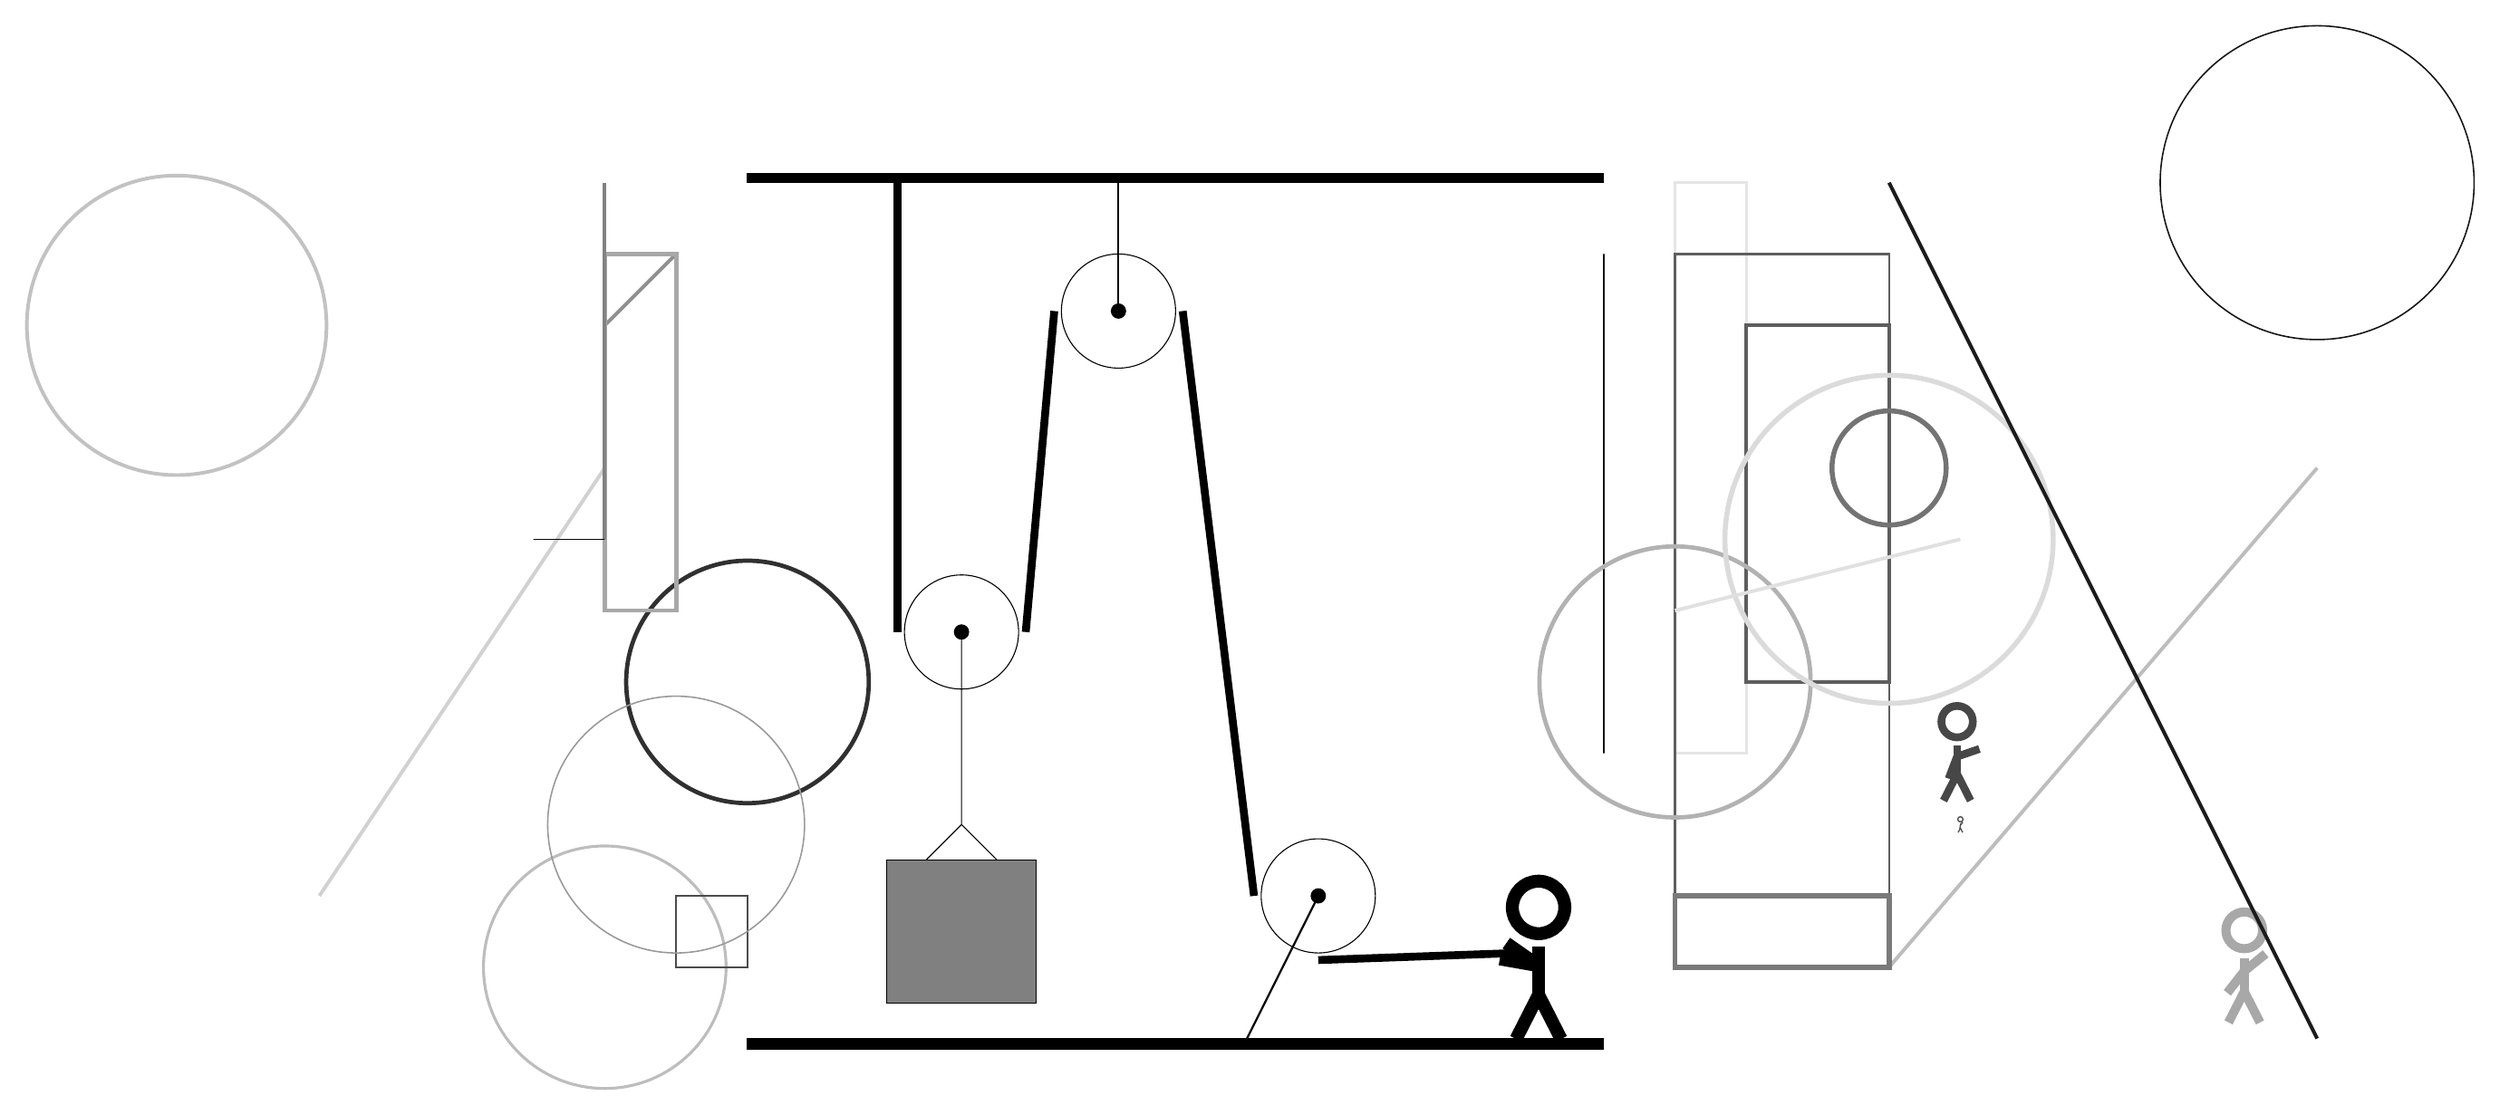
\begin{tikzpicture}
			%%%%% START %%%%%
			
			\draw[fill=black] (-2, 9) rectangle (10, 9.125);
			
			\draw (3.2, 7.2) circle (0.8);
			\draw[fill=black] (3.2, 7.2) circle (0.1);
			\draw[thick] (3.2, 7.2) -- (3.2, 9);
			
			\draw (6, -1) circle (0.8);
			\draw[fill=black] (6, -1) circle (0.1);
			\draw[thick] (6, -1) -- (5, -3);
			
			\draw (1, 2.7) circle (0.8);
			\draw[fill=black] (1, 2.7) circle (0.1);
			
			\draw (1, 2.7) -- (1, 0) -- (0.5, -0.5);
			\draw (1, 0) -- (1.5, -0.5);
			\draw[fill=black!50] (-0.05, -0.5) rectangle (2.05, -2.5);
			
			\draw[line width=0.4mm, color=black!10] (11, 1) rectangle (12, 9);
			
			\draw [line width=0.4mm, color=black!26](-4, -2) circle (1.7);
			\draw[line width=0.5mm, color=black!44](-4, 7) -- (-3, 8);
			\draw [line width=0.6mm, color=black!81](-2, 2) circle (1.7);
			
			\draw[line width=0.5mm, color=black!63] (12, 7) rectangle (14, 2);
			\draw[line width=0.5mm, color=black!26](14, -2) -- (20, 5);
			
			\draw[line width=0.6mm, color=black!34] (-4, 3) rectangle (-3, 8);
			
			\draw[line width=0.2mm, color=black!70] (-3, -1) rectangle (-2, -2);
			\draw [line width=0.2mm, color=black!92](20, 9) circle (2.2);
			
			\draw[line width=0.3mm, color=black!63] (11, -2) rectangle (14, 8);
			\draw [line width=0.5mm, color=black!24](-10, 7) circle (2.1);
			
			\draw[line width=0.3mm, color=black!93] (10, 1) rectangle (10, 8);
			\draw [line width=0.6mm, color=black!30](11, 2) circle (1.9);
			
			\draw [line width=0.7mm, color=black!55](14, 5) circle (0.8);
			\draw [line width=0.7mm, color=black!14](14, 4) circle (2.3);
			\draw [line width=0.2mm, color=black!40](-3, 0) circle (1.8);
			
			\draw[line width=0.5mm, color=black!18](-4, 5) -- (-8, -1);
			
			\node[line width=0.3mm, color=black!68] at (15, 0) {\Strichmaxerl[1][83][52]};
			\draw[line width=0.2mm, color=black!98] (-4, 4) rectangle (-5, 4);
			
			\draw[line width=0.5mm, color=black!49](-4, 4) -- (-4, 9);
			\node[line width=0.3mm, color=black!34] at (19, -2) {\Strichmaxerl[7][52][39]};
			
			\draw[line width=0.5mm, color=black!89](14, 9) -- (20, -3);
			
			\draw[line width=0.5mm, color=black!12](15, 4) -- (11, 3);
			\draw[line width=0.7mm, color=black!52] (11, -2) rectangle (14, -1);
			\node[line width=0.4mm, color=black!72] at (15, 1) {\Strichmaxerl[6][69][19]};
			
			\draw [line width=0.3mm, color=black!68](11, 6) circle (0.0);
			
			\draw[line width=1.1mm] (0.1, 9) -- (0.1, 2.7);
			\centerarc[line width=1.1mm](1, 2.7)(180:360:0.9);
			\draw[line width=1.1mm](1.9, 2.7) -- (2.3, 7.2);
			\centerarc[line width=1.1mm](3.2, 7.2)(0:180:0.9);
			\draw[line width=1.1mm](4.1, 7.2) -- (5.1, -1);
			\centerarc[line width=1.1mm](6, -1)(180:270:0.9);
			\draw[line width=1.1mm](6, -1.9) -- (8.8, -1.8);
			
			\node at (9, -1.9) {\Strichmaxerl[10][-35][170]};
			
			\draw[fill=black] (-2, -3) rectangle (10, -3.15);
			
			%%%%% END %%%%%
		\end{tikzpicture}
	\end{figure}	
\end{document}